\chapter{Effects}

While the digital revolution made it possible to create popular effects like Echos, Flangers or Reverbs more efficiently using logic circuits and digital signal processing, most effects found in digital synthesizers today have a long history of analog implementation. Rock stars like Jimi Hendrix, famous for using the "Wah-Wah" effect, applied effects to their sound long before digitization. The following sections will describe four common effects and explain their implementation.

\section{Delay Lines and the Delay Effect}

Delay lines store samples and \emph{delay} their retrieval by a certain number of sample times. Just like delay lines are at the foundation of many digital filters, they are also the primary building block of a great number of different effects. Consequently, they must be examined and discussed thoroughly before attempting to create any other digital effects. However, having a well-founded understanding of delay lines also makes the implementation of many effects a trivial task. It should be noted that when a delay line is used as an effect simply to delay samples, it will be referred to as a "Delay" effect.

\subsection{Simple Delay Lines}

\noindent  If the time by which a sample is delayed is constant for each sample, a delay line can be implemented using a simple First-In-First-Out (FIFO) data-structure such as a Queue. Figure \ref{fig:simpledelay} visualizes such a delay line and Table \ref{code:simpledelay} shows a C++ implementation. \citebs{118}

\begin{figure}[h!]
  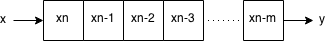
\includegraphics[scale=0.8]{img/simpledelay}
  \caption{Visualization of a simple FIFO delay line.}
  \label{fig:simpledelay}
\end{figure}

\begin{table}[t!]
  \code{simpledelay.cpp}
  \caption{A C++ class that implements a very simple delay line of fixed size.}
  \label{code:simpledelay}
\end{table}

\pagebreak

\subsection{Flexible Delay Lines}

While simple delay lines are easy to implement, they are not efficient if the delay time is not constant, as changing the size would require the re-allocation of memory to suit the new size and subsequent copying of all items from the old delay line into the new one. Moreover, the moving of all samples by one index after retrieving the latest output sample is highly inefficient, especially for long delay times. A more reasonable approach is to implement a delay line as a circular buffer with a fixed maximum length and then to vary the distance between a read and a write iterator relative to the current delay time. The circularity is achieved by wrapping the read or the write index back to the front of the buffer if either reaches the end. Figure \ref{fig:ringdelay} shows such a circular buffer in an abstract visualization, where the write iterator, which points to the position where incoming samples are stored into the delay line, is currently at index 0. The Figure also shows two possible positions of the read iterator, from which delayed samples are retrieved, which both result in a different delay time. It should be noted that read iterator A and B do not exist simultaneously, they just show possible indices for the read iterator. Read position A would cause a delay of 5 sample times while read position B would result in a 20 sample delay. Figure \ref{fig:seqdelay} shows the same buffer and iterators in a more realistic sequential layout, as it is stored in computer memory.

\begin{figure}[p!]
  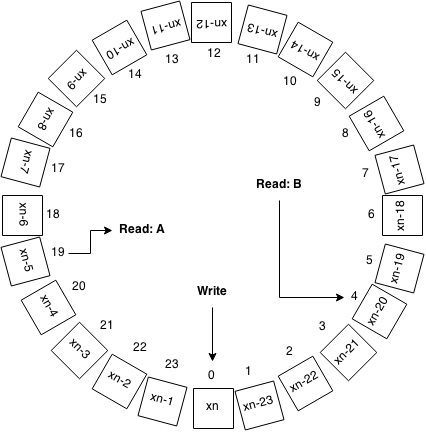
\includegraphics[scale=0.7]{img/ringdelay}
  \caption{A circular delay buffer with two different possible read positions A and B. The labels inside the boxes are the relative sample delays and the labels outside the boxes are the sequential indices. The write iterator is where new samples are stored and the read iterators are where delayed samples are retrieved from.}
  \label{fig:ringdelay}
\end{figure}

\begin{figure}[p!]
  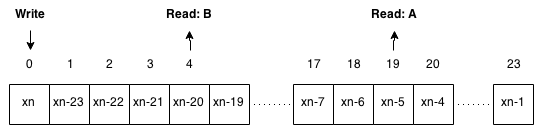
\includegraphics[scale=0.7]{img/seqdelay}
  \caption{The buffer from Figure \ref{fig:ringdelay} in a sequential layout.}
  \label{fig:seqdelay}
\end{figure}

\subsection{Interpolation}

It is also possible to have fractional delay values if samples are interpolated. Equation \ref{eq:interpolatedelay} shows how this interpolation process is performed, where $i$ is the integral and $f$ the fractional portion of the $n$-sample delay. Note that this is the same interpolation algorithm that is performed to retrieve sample values from fractional Wavetable indices.

\begin{equation}
  y_{n} = x_{i} + ((x_{i-1} - x_{i}) \cdot f)
  \label{eq:interpolatedelay}
\end{equation}

\subsection{Feedback and Decay}

Two parameters commonly associated with delay lines are \emph{feedback} and \emph{decay}. The feedback control of a delay line determines how much of the output signal is fed back into the delay line together with the input signal. The decay parameter determines the level of attenuation of the output signal as it leaves the delay line. It is "[...] applied each time the [fed-back] sample travels through the delay line and is equivalent to the dampening, or decay, of a signal over time". When these two parameters are used together, such a delay line is called a "Resonator". Figure \ref{fig:resonator} shows a block diagram for such a resonator and Figure \ref{fig:resonatorwav} displays a sound wave resulting from a resonator. \citebs{120}

\begin{figure}
  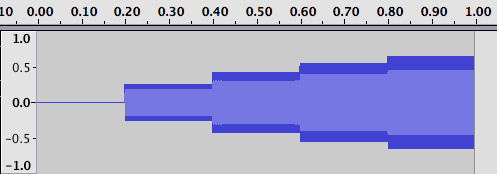
\includegraphics[scale=0.6]{img/resonatorwav}
  \caption{A sound wave resulting from a resonator. The initial silence is caused by the delay line filling up and delayed samples consequently still being equal to 0. The increase in amplitude per delay time (200 ms) is due to the feedback control. Because the decay is not 0, the amplitude does not double per delay time as it would if there were no decay and full feedback. Rather, the sound decays with time and would reach its maximum after 4 seconds.}
  \label{fig:resonatorwav}
\end{figure}

\begin{figure}
  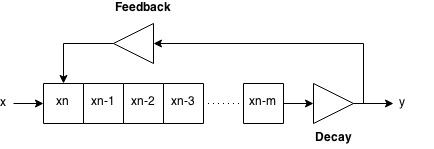
\includegraphics[scale=0.7]{img/resonator}
  \caption{A resonating delay line.}
  \label{fig:resonator}
\end{figure}

\subsection{Dry/Wet Control}

Almost every effect, including the Delay effect, has what is called a "dry/wet" control. If the dry signal is the unchanged input signal and the wet signal the fully processed output signal, the dry/wet control determines how much of an effect is applied to the dry signal. Equation \ref{eq:drywet} gives a mathematical definition for this principle, where $dw$ is the dry/wet value between 0 (no effect) and 1 (full effect), $x_{n}$ the unchanged, "dry", input sample and $y_{n}$ the "wet" output signal from the effect.

\begin{equation}
  z_{n} = (x_{n} \cdot (1 - dw)) + (y_{n} \cdot dw)
  \label{eq:drywet}
\end{equation}

\subsection{Implementation}

In the synthesizer created for this thesis, a flexible delay line with all the properties and controls just mentioned is implemented in the \texttt{Delay} class. Relevant processing and updating methods of the \texttt{Delay} class are shown in Table \ref{code:delay}.

\begin{table}[thb!]
  \code{delay.cpp}
  \caption{Relevant member functions of the \texttt{Delay} class that implements a flexible delay line with feedback, decay, interpolation and dry/wet control.}
  \label{code:delay}
\end{table}

\pagebreak

\section{Echo}

The first effect that can be implemented very easily using just delay lines is the Echo effect. It is the result of summing an input sample with the output sample of a delay line. An implementation from the \texttt{Echo} class, derived from the \texttt{Delay} class, is shown in Table \ref{code:echo}.

\begin{table}[h!]
  \code{echo.cpp}
  \caption{The \texttt{process} method of the \texttt{Echo} class. This shows that an Echo is just the input sample summed with the output from the delay line.}
  \label{code:echo}
\end{table}

\section{Flanger}

A Flanger effect is created by mixing a signal with a delayed version of itself and varying the time by which it is delayed with a Low Frequency Oscillator. The middle delay time around which the LFO oscillates is called the "center" value. The term "depth" is used for the value that is added to or subtracted from the center value periodically. For example, if the center value is 10 ms and the depth 4 ms, the delay time will oscillate between 6 ms and 14 ms. The "rate" parameter controls how fast the LFO oscillates. A Flanger's "feedback" control is not the same as for delay lines, as it does not control how much of the output signal is fed back into the delay line. Rather, the feedback value determines how much of the sample at the center delay value is subtracted from the input sample. Varying the feedback controls the coloration and brightness of the sound produced. Lastly, a Flanger also has a dry/wet parameter, whose function was already described. Figure \ref{fig:flanger} depicts a block diagram for a Flanger. The sound produced by a Flanger effect can be described as a "swooshing" sound. \citebs{136} Table \ref{code:flanger} shows the \texttt{Flanger} class' \texttt{process} method.

\begin{figure}[p!]
  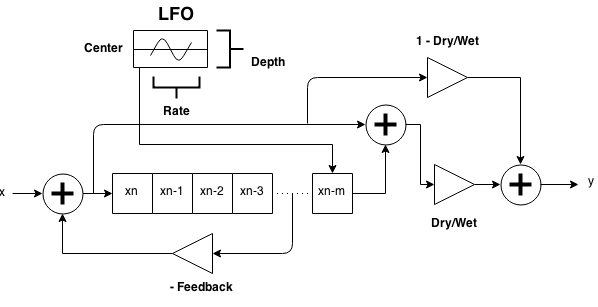
\includegraphics[scale=0.7]{img/flanger}
  \caption{Block diagram for a Flanger effect. The LFO controls the delay length. The feedback is negative because it is subtracted from the input sample. }
  \label{fig:flanger}
\end{figure}

\begin{table}[p!]
  \code{flanger.cpp}
  \caption{Member function of the \texttt{Flanger} class that implements flanging.}
  \label{code:flanger}
\end{table}

\section{Reverb}

When a musician plucks a string on his guitar or bangs a percussion drum in a closed room, the sound that reaches a listener's ears does not stem solely from the sound's source. Rather, the sound emited from the musical instrument reflects off the room's walls and ceiling as well as any other object it meets on the way to the listener. This mixture of original and reflectd sound is called reverberation \citebs{129}. Naturally, the degree of reverberation depends, among other things, to a large part on the space of the room in which the sound is emitted. For example, an organ will sound differently if played in a large cathedral than it will in a small classroom. Therefore, any parameters that control the degree of reverberation essentially determine the size of the "virtual room" in which the sound is played. Most reverberators, reverbs for short, allow the user to control the reverb "time" and the reverb "rate". The reverb time determines how long it takes for the sound to reach inaudible levels, while the reverb rate controls at what rate this fading out occurs. Finally, there is also a dry/wet control as for all other effects as well.

\subsection{Schroeder Reverb}

A relatively well-known and moderately popular reverb algorithm is the so-called "Schroeder Reverb", which consists of four parallel delay lines whose signals are fed into two all-pass filters connected in series. Figure \ref{fig:reverb} depicts a block diagram for a Schroeder Reverb. To simulate how sound waves reflect off different surfaces in a room, the delay lines are given different lengths. The decay parameter of these delay lines is determined by the reverb time and rate. The Schroeder Reverb's all-pass filters have fixed delay times and decay values. Table \ref{tb:reverb} gives these various delay line lengths and decay values. \citebs{133}

\begin{figure}[hb!]
  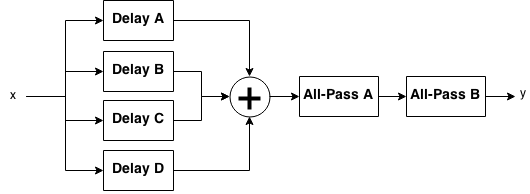
\includegraphics[scale=0.7]{img/reverb}
  \caption{Block diagram for a Schroeder Reverb effect.}
  \label{fig:reverb}
\end{figure}

\begin{table}[hb!]

  \centering

  \begin{tabular}[]{ | c | c | c |}
    \hline
    \rowcolor[gray]{0.8}
    Component & Delay Time & Decay Value \\\hline
    Delay A & 0.0297 & Variable\\\hline
    Delay B & 0.0371 & Variable \\\hline
    Delay C & 0.0411 & Variable \\\hline
    Delay D & 0.0437 & Variable \\\hline
    All-Pass A & 0.09638 & 0.0050 \\\hline
    All-Pass B & 0.03292 & 0.0017\\
    \hline
  \end{tabular}

  \caption{Delay times and decay values for a Schroeder Reverb.}

  \label{tb:reverb}

\end{table}

\pagebreak

\subsection{Implementation}

Table \ref{code:reverb} shows relevant member of function of the \texttt{Reverb} class, which implements a Schroeder Reverb.

\begin{table}[h!]
  \code{reverb.cpp}
  \caption{This code exerpt from the \texttt{Reverb} class shows how the Schroeder Reverb's delay lines and all-pass filters are initialized and then used to reveberate a signal.}
  \label{code:reverb}
\end{table}
